\documentclass{beamer}
\usepackage{graphics}
\usepackage{epsfig}
\usepackage{multicol}
\setbeamertemplate{navigation symbols}{}
\newcommand{\RR}{\ensuremath{\mathbb{R}}}
\newcommand{\NN}{\ensuremath{\mathbb{N}}}
\newcommand{\QQ}{\ensuremath{\mathbb{Q}}}
\newcommand{\CC}{\ensuremath{\mathbb{C}}}
\newcommand{\ZZ}{\ensuremath{\mathbb{Z}}}
\newcommand{\TT}{\ensuremath{\mathbb{T}}}
\DeclareMathOperator{\Min}{Min}
\DeclareMathOperator{\Dom}{Dom}
\DeclareMathOperator{\vol}{vol}
\DeclareMathOperator{\Aut}{Aut}
\DeclareMathOperator{\Stab}{Stab}
\DeclareMathOperator{\Sym}{Sym}
\DeclareMathOperator{\Grp}{Grp}
\DeclareMathOperator{\GL}{GL}
\DeclareMathOperator{\Id}{Id}

\begin{document}
\title{Bathymetry smoothing in ROMS: A new approach}
\author{
{\small
\begin{multicols}{2}
\textcolor{red}{\large Mathieu Dutour Sikiri\'c}\\[2mm]
\textcolor{red}{\large Ivica Janekovi\'c}\\[2mm]
\end{multicols}
\begin{center}
\textcolor{red}{\large Milivoj Kuzmi\'c}\\[2mm]
\textcolor{red}{Institute Rudjer Bo\u skovi\'c, Zagreb}
\end{center}
}
}
%\date{\today} 
\date{\empty}

\frame{\titlepage} 

\frame{
  \frametitle{PLAN}

\begin{itemize}
\item[I]   Problem set up\\[1cm]
\item[II]  Solution approaches\\[1cm]
\item[III] Comparison of selected methods
\end{itemize}
}


\frame{
\begin{center}
\begin{tabular*}{7cm}{c}
\\[-0.5cm]
{\Huge
\textcolor{blue}{I. }\textcolor{red}{Problem set up}
}
\end{tabular*}
\end{center}
}


\frame{
  \frametitle{Sigma coordinate systems}

\begin{itemize}
\item One way to deal with varying bathymetry: use $\sigma$-coordinates (\textcolor{blue}{Phillips 1957})
\begin{center}
\begin{minipage}[b]{24mm}
\centering
\resizebox{26mm}{!}{\rotatebox{0}{\includegraphics{OceanPic/SigmaCoordSec.pdf}}}\par
\end{minipage}
\end{center}
\item On every cell $e$ of bathymetry $h(e)$, choose a number $N$ of vertical levels $h(e,k)$ for $1\leq k\leq N$ with $h(e,0)=h(e)$ and $h(e,N)=0$.
%\item[\textcolor{red}{\ding{224}}] Phillips, N.A., 1957. {\em A coordinate system having some special advantages for numerical forecasting}. Journal of Meteorology 14, 184--185.
\item The differentiation rule of functions in $\sigma$-coordinate is
\begin{equation*}
\left.\displaystyle\frac{\partial f}{\partial x}\right|_z=\left.\displaystyle\frac{\partial f}{\partial x}\right|_{\sigma}+\frac{\partial h}{\partial x} \frac{\partial f}{\partial \sigma}
\end{equation*}
\item This creates a problem for horizontal derivatives, which become a difference of two terms.
The wrong computation of the \textcolor{red}{horizontal pressure gradient} creates artificial currents.
\item \textcolor{blue}{Smagorinsky 1967},
\textcolor{blue}{Janji\'c 1977},
\textcolor{blue}{Mesinger 1982},
\textcolor{blue}{Haney 1991}
\end{itemize}
}


%\frame{
%  \frametitle{Pressure gradient problem}
%
%\begin{itemize}
%\item The differentiation rule of functions in $\sigma$ coordinate is
%\begin{equation*}
%\left.\displaystyle\frac{\partial f}{\partial x}\right|_z=\left.\displaystyle\frac{\partial f}{\partial x}\right|_{\sigma}+\frac{\partial h}{\partial x} \frac{\partial f}{\partial \sigma}
%\end{equation*}
%\item This is creates problem for the computation of the horizontal pressure gradient since the derivative $\frac{\partial p}{\partial x}$ becomes a difference of two terms of same sign.
%\item This is a very old problem (Smagorinsky 1967, Mesinger 1982, Haney 1991).
%\end{itemize}
%}



\frame{
  \frametitle{The roughness factors}

\begin{itemize}
\item If $e$ and $e'$ are two adjacent wet cells, then
\begin{equation*}
rx_0(h, e,e')= \frac{|h(e)-h(e')|}{h(e)+h(e')}
\end{equation*}
The maximum over all such pairs is $rx_0(h)$, i.e. the
\textcolor{red}{Beckman \& Haidvogel number}.
\item If the vertical levels of the bathymetries are $h(e,k)$ for $1\leq k\leq N$ then
\begin{equation*}
rx_1(h, e,e',k)=\frac{|h(e,k)-h(e',k)+h(e,k-1)-h(e',k-1)|}{h(e,k)+h(e',k)-h(e,k-1)-h(e',k-1)}.
\end{equation*}
The maximum over $k$ and pairs $e$, $e'$ of adjacent wet cells is $rx_1(h)$.\\
This number is named \textcolor{red}{hydrostatic instability number} or \textcolor{red}{Haney number}.
\end{itemize}
}



\frame{
  \frametitle{Hydrostatic stability}

\begin{itemize}
\item Denote by $C_k(e)$ the parallelepiped of water between depth $h(e,k-1)$ and depth $h(e,k)$.
\item \textcolor{red}{Hydrostatic stability} means that if $e$ and $e'$ are any two adjacent cells, then $C_k(e)$ and $C_k(e')$ share a level.
\begin{center}
\begin{minipage}[b]{50mm}
\centering
\resizebox{36mm}{!}{\rotatebox{0}{\includegraphics{OceanPic/HydrostaticInconsistency.pdf}}}\par
\end{minipage}
\end{center}
\item To impose that $C_k(e)$ and $C_k(e')$ share a level is equivalent to $rx_1(h, e, e', k)\leq 1$ (\textcolor{blue}{Rousseau and Pham 1971}, \textcolor{blue}{Mesinger 1982}, \textcolor{blue}{Haney 1991}).
\item This requirement is very strong and almost impossible to fulfill.
\end{itemize}
}



\frame{
  \frametitle{Vertical parametrization in ROMS}
\begin{itemize}
\item The ROMS vertical parametrization depends on three parameters $hc$, $\theta_s$, $\theta_b$
\begin{equation*}
h(e,k)=s_w(k) hc + (h(e) - hc) C_w(k).
\end{equation*}
$hc$ is the thermocline parameter and it is lower than the minimal
depth of the model.
\item The vertical parametrization function depends on $\theta_s$ and $\theta_b$ and is $s_w(k)=\frac{N-k}{N}$.
\begin{equation*}
C_w(k)=(1-\theta_b)\frac{\sinh \theta_s s_w(k)}{\sinh \theta_s}
+\theta_b \left\{\frac{1}{2} + \frac{\tanh \theta_s(s_w(k) - \frac{1}{2})}{2 \tanh \frac{\theta_s}{2}}\right\}
\end{equation*}
This formula is relatively arbitrary (\textcolor{blue}{Song 1994}) and another one may work just as well.
\item If $hc=0$ then we have $h(e,k)=h(e)C_w(k)$ and we get
\begin{equation*}
rx_1(h)=\max_{1\leq k\leq N} \frac{C_w(k) + C_w(k-1)}{C_w(k) - C_w(k-1)} rx_0(h)
\end{equation*}
%\item[\textcolor{red}{\ding{224}}]
%Song, Y., Haidvogel, D.B., 1994.
%{\em A semi-implicit ocean circulation model using a generalized topography-following coordinate system}.
%Journal of Computational Physics 115, 228--244.
\end{itemize}
}





\frame{
  \frametitle{What are the right parameters?}

There is no general agreement on this question
\begin{itemize}
\item The parameters $\theta_s$, $\theta_b$ have to be chosen to represent
correctly the vertical structure.
\item The factor which matters for the horizontal pressure gradient is the Haney number $rx_1(h)$.
\item It is extremely difficult to achieve $rx_1(h)\leq 1$.
\item In \textcolor{blue}{Mellor-Ezer-Oey 1994} it is argued that the HPG error is not very important and disappears after running the model for some time.
\item \textcolor{blue}{Kliem-Pietrzak, 1999} contests this for the Skagerrak region.
\item \textcolor{blue}{Sasha Shchepetkin, 2008} says that $rx_1(h)\leq 3$ is ``safe'', $rx_1(h)\simeq 5$ is ``common'' and $rx_1(h)\geq 8$ is ``insane''.
\item \textcolor{blue}{Kate Hedstrom, 2008} reported no problem with $rx_1(h)\simeq 16$.
%\item There are contrary argument about the importance of pressure gradient error by \textcolor{blue}{Mellor-Ezer-Oey 1994} and \textcolor{blue}{Kliem-Pietrzak, 1999}.
\item We experienced blow ups with grids with $rx_1(h)\geq 10$.
\end{itemize}
}



\frame{
  \frametitle{Possible ways to deal with the problem}

If the bathymetry is too steep then this causes instabilities and inaccuracies.
Some possible ways to deal with it:
\begin{itemize}
\item Use a high order pressure gradient scheme (\textcolor{blue}{Chu \& Fan, 1997, 1998, 2003})
(\textcolor{red}{computational price})
\item Adjust the vertical stratification, i.e. $s_w$, $C_w$ and in case of ROMS $\theta_s$, $\theta_b$.
\item Decrease the number $N$ of vertical levels (\textcolor{red}{less realistic})
\item Make the horizontal grid finer (\textcolor{red}{computational price}).
\item Smooth the bathymetry (\textcolor{red}{less realistic}).
\item Use a $z$- or generalized coordinate system (\textcolor{red}{change of model}).
\end{itemize}
We consider the smoothing methods to reduce the magnitude of the problem.
}




\frame{
\begin{center}
\begin{tabular*}{7cm}{c}
\\[-0.5cm]
{\Huge
\textcolor{blue}{II. }\textcolor{red}{Solution approaches}
}
\end{tabular*}
\end{center}
}


\frame{
  \frametitle{The goal}

\begin{itemize}
\item The grid is build in the following way:
\begin{itemize}
\item Build an initial grid using coastline informations.
\item Choose the parameters $\theta_s$, $\theta_b$ and $hc$.
\item Interpolate the initial bathymetry $h^{obs}$ from existing data set (NOAA, Gshhs, Gebco, etc.)
\item Determine the smoothed bathymetry $h$.
\end{itemize}
\item Requirements:
\begin{itemize}
\item $rx_0(h)$ and $rx_1(h)$ low.
\item The ``distance'' between $h$ and $h^{obs}$ small.
\item $h$ should have the same physical characteristics as $h^{obs}$.
\end{itemize}
\item For a given $r$ and $h^{obs}$, we will present methods to get $h$
with $rx_0(h) \leq r$.
\item The analysis for $rx_1$ works similarly.
\end{itemize}
}


\frame{
  \frametitle{The Shapiro filter}

\begin{itemize}
\item It is a filter designed to smooth out fast waves in finite
difference models (\textcolor{blue}{Shapiro 1975}).
\item It is applied to the bathymetry in the following way:
\begin{flushleft}
$h \textcolor{red}{\leftarrow} h^{obs}$\\
\textbf{while} $rx_0(h) > r$ \textbf{do}\\
\hspace{2ex} $h' \textcolor{red}{\leftarrow}$ Shapiro filtering of $h$ on $x$ direction.\\
\hspace{2ex} \textbf{for} $e$ in wet cells \textbf{do}\\
\hspace{2ex} \hspace{2ex} \textbf{if } $rx_o(h, e)>r$ \textbf{then}\\
\hspace{2ex} \hspace{2ex} \hspace{2ex} $h(e) \textcolor{red}{\leftarrow} h'(e)$\\
\hspace{2ex} \hspace{2ex} \textbf{end if}\\
\hspace{2ex} \textbf{end for}\\
\hspace{2ex} Do the same in $y$ direction\\
\textbf{end do}
\end{flushleft}
\item For some bathymetries the Shapiro filter converges to $h$ with $rx_0(h) > r$ and thus the program never ends.
\end{itemize}
}


\frame{
  \frametitle{Laplacian filter}

\begin{itemize}
\item It works in the following way:
\begin{itemize}
\item start with $h=h^{obs}$.
\item If $rx_0(h, e) > r$ we do:
\begin{equation*}
h(e)\textcolor{red}{\leftarrow} h(e)+\frac{1}{2N(e)} \sum_{e'\in N(e)} \{ h(e')-h(e)\}
\end{equation*}
with $N(e)$ the set of wet cells adjacent to the wet cell $e$.
\item Iterate until $rx_0(h)\leq r$.
\end{itemize}
\item This filter is more stable than Shapiro filter, but there is a still a problem of having the program end.
\item Shapiro filter and Laplacian filter are very frequently used but they are not very good methods.
\end{itemize}
}


\frame{
  \frametitle{The Martinho \& Batteen scheme}

\begin{itemize}
\item Whenever the the roughness is not correct the chose solution
(\textcolor{blue}{Martinho \& Batteen 2006}) is to
increase the bathymetry.
\begin{itemize}
\item Start with $h=h^{obs}$
\item If
\begin{equation*}
\frac{h(e) - h(e')}{h(e) + h(e')} > r\quad{\rm then} \quad h(e')\textcolor{red}{\leftarrow} \frac{1-r}{1+r}h(e)
\end{equation*}
\item All pairs $(e, e')$ are considered iteratively until the slope factor is correct. The result is independent of the order of operations.
\end{itemize}
%\item[\textcolor{red}{\ding{224}}] Martinho, A.S., Batteen, M.L., 2006. {\em On reducing the slope parameter in terrain following numerical ocean models}. Ocean Modelling 13, 166--175.
\item They also proposed to preserve the volume by replacing the bathymetry $h$ obtained by their method by 
\begin{equation*}
h\textcolor{red}{\leftarrow} h \frac{\vol h^{obs}}{\vol h}
\end{equation*}
\item \textcolor{red}{Note}: the strategy of reducing the bathymetry does not work efficiently.
\end{itemize}
}




\frame{
  \frametitle{The Mellor-Ezer-Oey scheme}

\begin{itemize}
\item (\textcolor{blue}{Mellor 1994}) If we want to preserve volume, then another scheme is possible.
\begin{itemize}
\item If we have 
\begin{equation*}
\frac{h(e) - h(e')}{h(e) + h(e')} > r
\end{equation*}
then we write
\begin{equation*}
h(e)\textcolor{red}{\leftarrow} h(e)-\delta\quad {\rm and}\quad h(e')\textcolor{red}{\leftarrow} h(e')+\delta
\end{equation*}
with $\delta$ adjusted so that  $\frac{h(e) - h(e')}{h(e) + h(e')}=r$.
\item All pairs $(e,e')$ of adjacent wet cells are considered iteratively until the bathymetry is correct.
\end{itemize}
\item A priori, the final bathymetry depends from the order of the operations.
%\item[\textcolor{red}{\ding{224}}] Mellor, G.L., Ezer, T., Oey, L.-Y., 1994. {\em The pressure gradient conundrum of Sigma coordinate Ocean models}. Journal of Atmospheric and Oceanic Technology 11, 1126--1134.
\end{itemize}
}


\frame{
  \frametitle{Linear programming methods}

\begin{itemize}
\item The inequality $rx_0(h, e, e')\leq r$ corresponds to two linear inequalities:
\begin{equation*}
-r (h(e) + h(e'))\leq h(e)-h(e') \leq r (h(e) + h(e'))
\end{equation*}
\item We introduce some auxiliary variable $\delta(e)$ with 
\begin{equation*}
|h(e)-h^{obs}(e)| \leq \delta(e) \quad {\rm i.e.}\quad \pm(h(e)-h^{obs}(e))\leq \delta(e)
\end{equation*}
\item And we minimize
\begin{equation*}
\sum_{e} \delta(e) \quad{\rm that~is} \quad \sum_e |h(e)-h^{obs}(e)|.
\end{equation*}
\item There are many possible variants, which are still in the linear programming paradigm:
\begin{itemize}
\item Preserve the total volume of the basin.
\item Have a different objective function.
\item Impose only positive/negative corrections at some points.
\item Impose maximum amplitude condition.
\end{itemize}
\end{itemize}
}


\frame{
  \frametitle{Definition}

\begin{itemize}
\item A \textcolor{red}{linear program} is the problem of maximizing a linear function $f(x)$ over a set ${\mathcal P}$ defined by linear inequalities (\textcolor{red}{polyhedral}).
\begin{equation*}
{\mathcal P}=\{ x\in \RR^d \quad{\rm such~that} \quad f_i(x) \geq b_i\}
\end{equation*}
with $f_i$ linear and $b_i\in \RR$.
%\item The sets ${\mathcal P}$ are called \textcolor{red}{polyhedral}.
\item The solution of linear programs is attained at vertices of ${\mathcal P}$.
\item There are two classes of solution methods:
\begin{center}
\begin{minipage}[b]{38mm}
\centering
\resizebox{30mm}{!}{\rotatebox{0}{\includegraphics{OceanPic/SimplexMethod.pdf}}}\par
Simplex method
\end{minipage}
\begin{minipage}[b]{38mm}
\centering
\resizebox{30mm}{!}{\rotatebox{0}{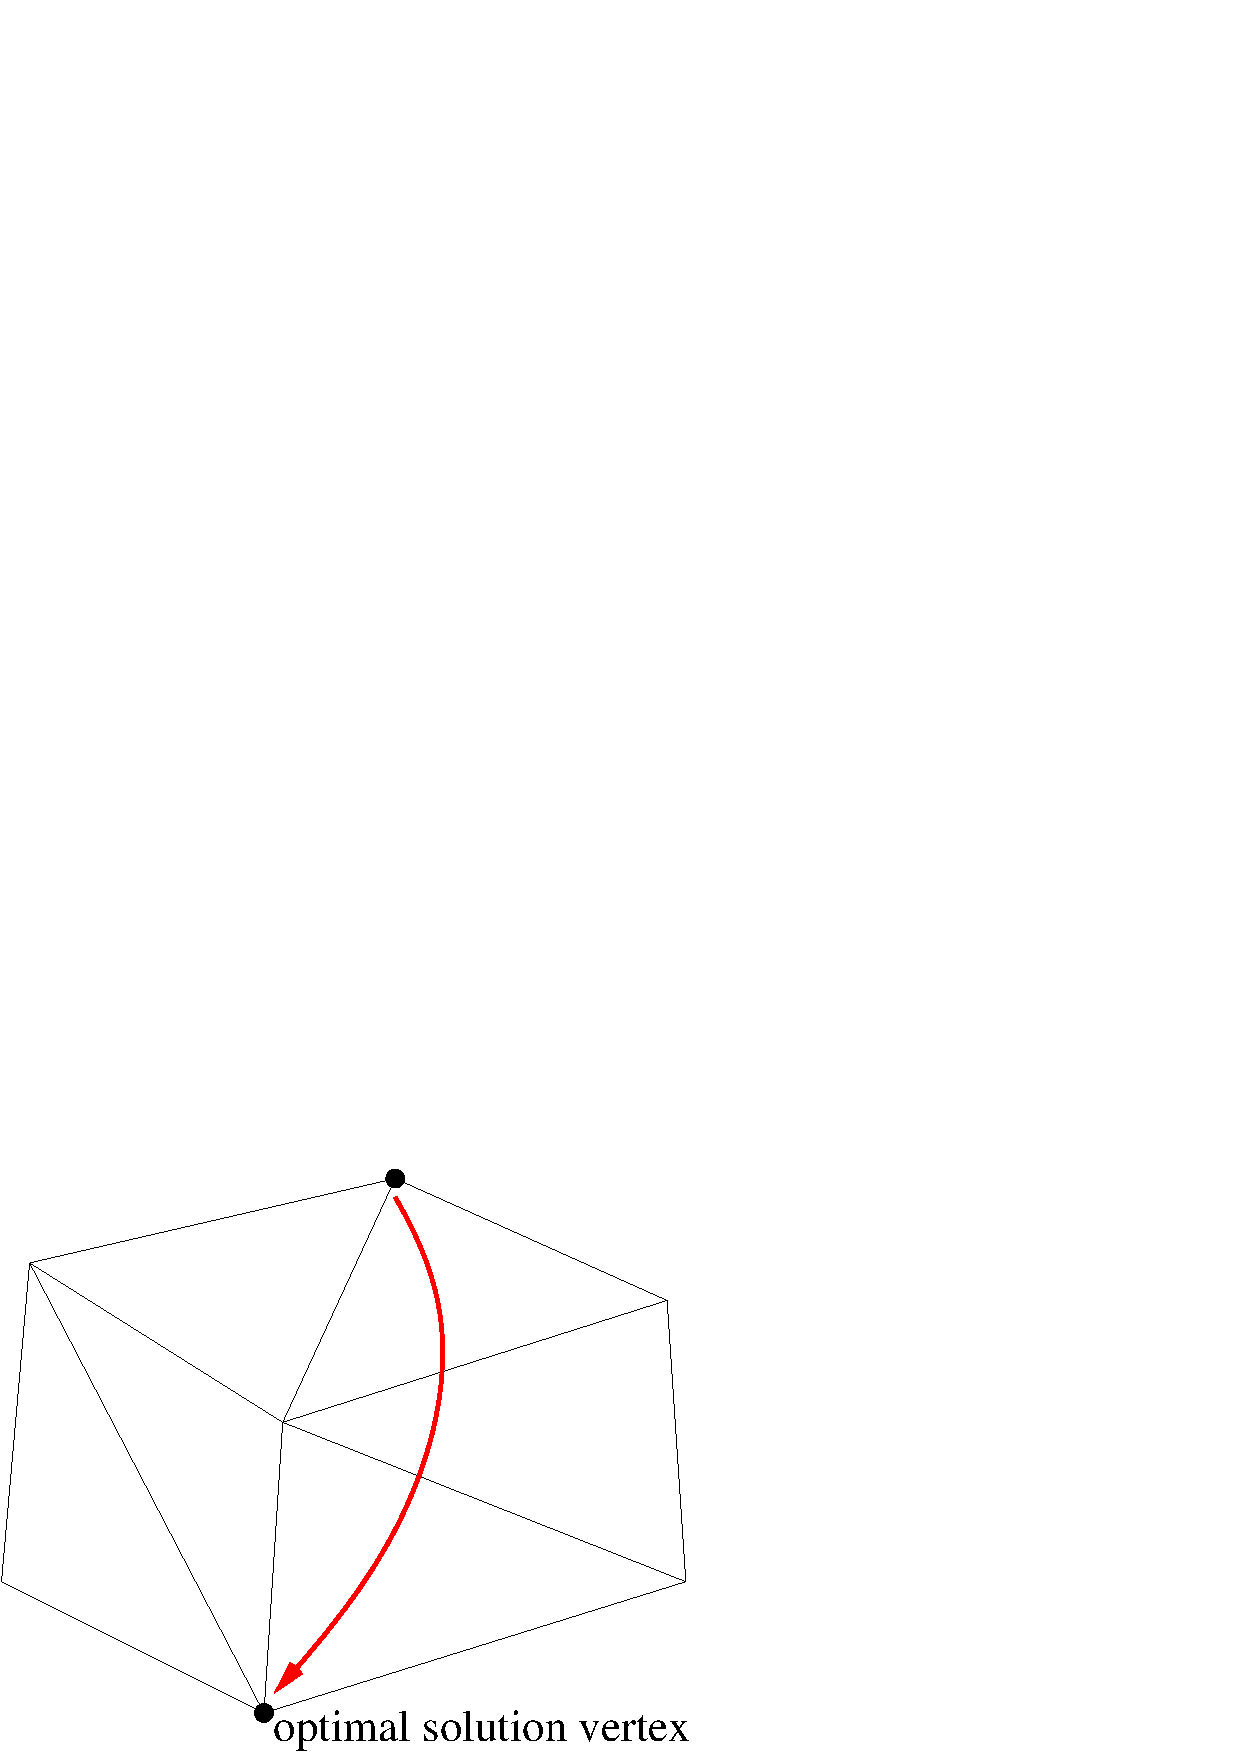
\includegraphics{OceanPic/InteriorPM.pdf}}}\par
Interior point method
\end{minipage}
\end{center}


\end{itemize}
}




%\frame{
%  \frametitle{Solution methods}
%
%\begin{itemize}
%\item There are two classes of solution method for solving linear programs:
%\item Simplex method (take one vertex and optimize step by step).
%\item Interior Point methods (take an interior point and make it nearer to the optimal solution)
%\end{itemize}
%}







\frame{
\begin{center}
\begin{tabular*}{7cm}{c}
\\[-0.5cm]
{\Huge \textcolor{blue}{III. }\textcolor{red}{Comparison}}\\
{\Huge \textcolor{red}{of selected methods}}
\end{tabular*}
\end{center}
}


\frame{
  \frametitle{The Adriatic Sea}
\begin{center}
\begin{minipage}{60mm}
\centering
\resizebox{60mm}{!}{\rotatebox{0}{\includegraphics[bb=63 226 398 567, clip]{OceanPic/RawBathyContourRect_V2_norect.pdf}}}
%RawBathyContourRect.pdf
\end{minipage}
\end{center}
\hspace{-2.7mm}\begin{itemize}
\item The bathymetry is highly varying and the coastline is diverse.
\item We chose three grids $160\times 60$, $127\times 368$, $271\times 751$
\end{itemize}
}



\frame{
  \frametitle{Regions of hydrostatic stability}

\begin{center}
\hspace{-1.1cm}\begin{minipage}[b]{3.8cm}
\centering
%\hspace{-1cm}
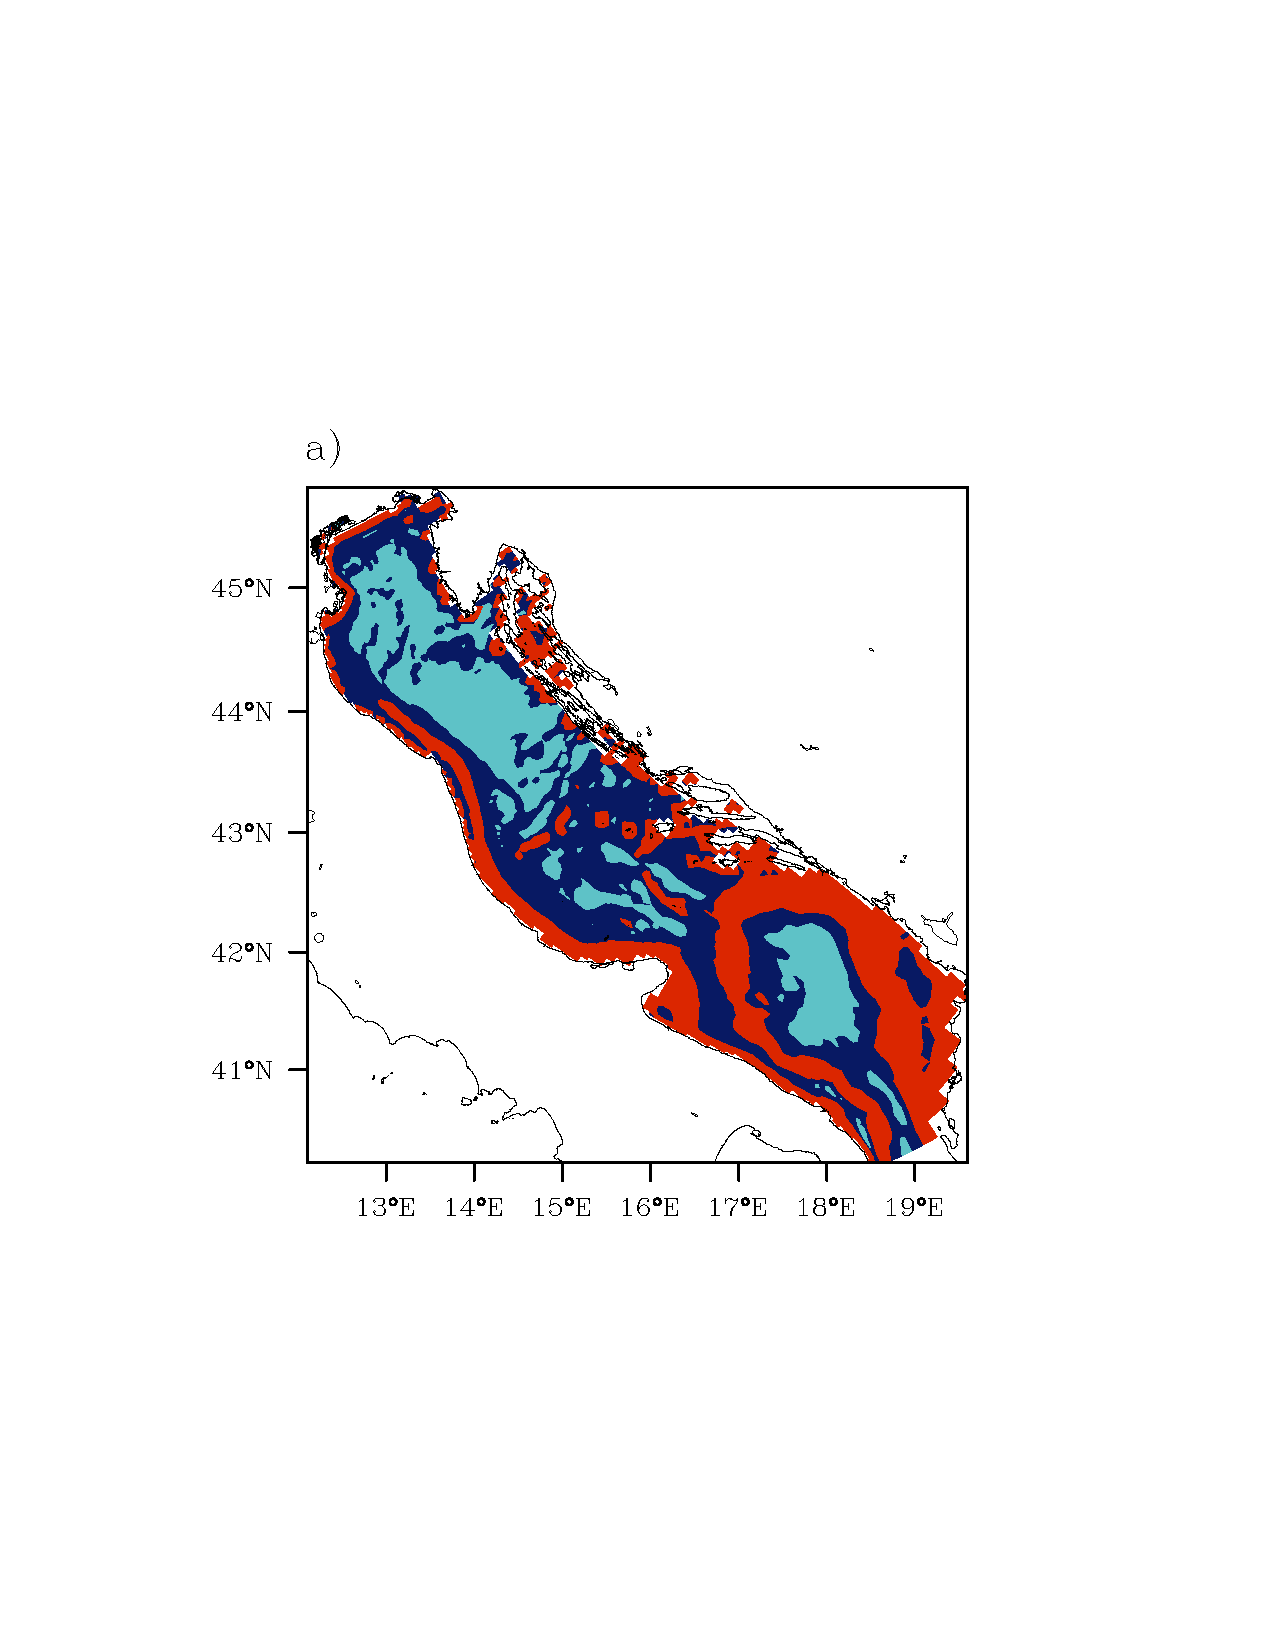
\epsfig{height=40mm, clip=, bb=100 209 465 560, file=OceanPic/ADRIA02_Hydrostatic.pdf}\par
$60\times 160$
\end{minipage}
\hspace{0.2cm}
\begin{minipage}[b]{3.7cm}
\centering
%\hspace{-0.5cm}
\epsfig{height=40mm, clip=, bb=145 209 465 560, file=OceanPic/NCOM2_Hydrostatic.pdf}\par
$127\times 368$
\end{minipage}
\hspace{0.1cm}
\begin{minipage}[b]{3.5cm}
\centering
\epsfig{height=40mm, clip=, bb=145 209 465 560, file=OceanPic/NCOM1_Hydrostatic.pdf}\par
$271\times 751$
\end{minipage}
\end{center}
The regions of hydrostatic consistency ($rx_1(h, e)\leq 1$ in light blue), hydrostatic inconsistency ($1\leq rx_1(h, e)\leq 5$ in dark blue) and hydrostatic instability ($rx_1(h, e)\geq 5$ in red)
}



\frame{
  \frametitle{Average amplitude of bathymetry modification}

\begin{center}
\begin{minipage}[b]{5.3cm}
\centering
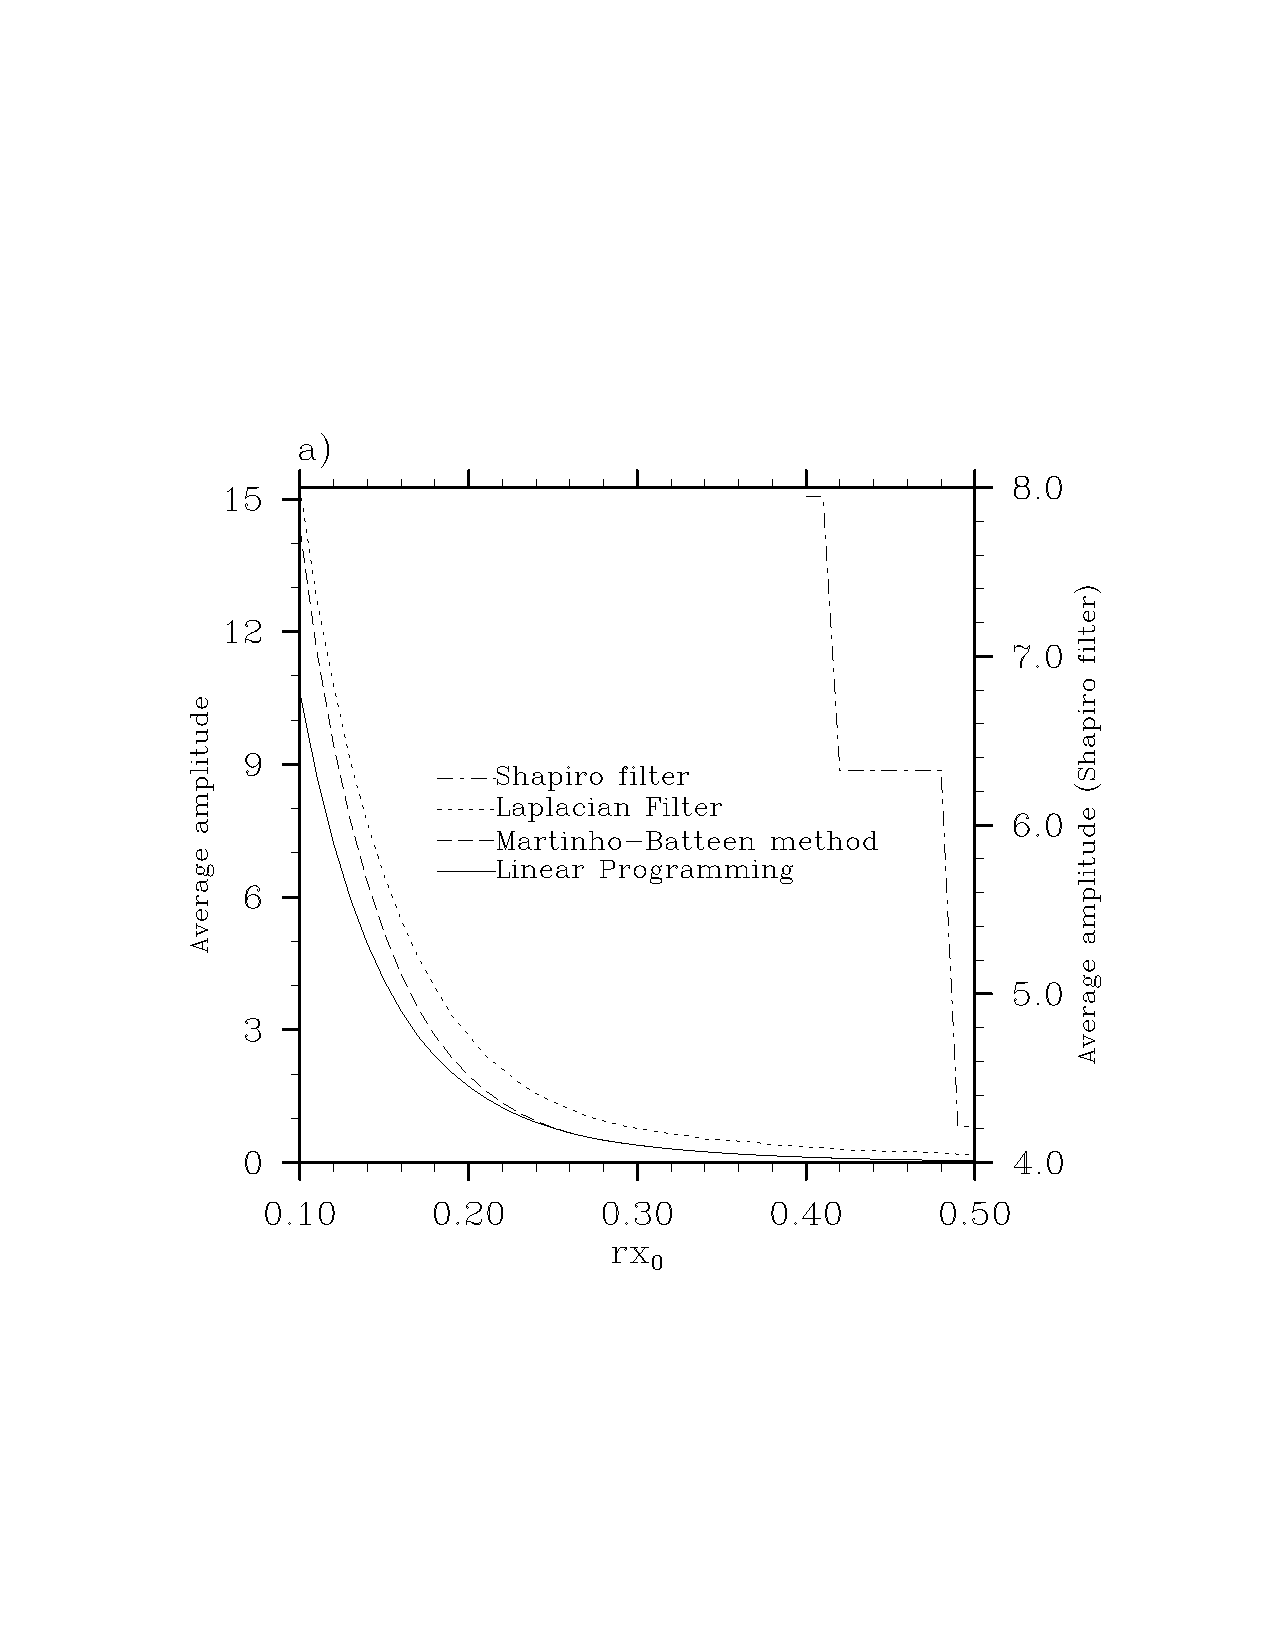
\epsfig{height=49mm, clip=, bb=90 182 510 566, file=OceanPic/ADRIA02_Various.pdf}\par
$60\times 160$
\end{minipage}
\begin{minipage}[b]{5.3cm}
\centering
\epsfig{height=49mm, clip=, bb=102 182 531 566, file=OceanPic/VER10_NCOM2_Various.pdf}\par
$127\times 368$
\end{minipage}
\end{center}
The average amplitude of bathymetry modification (m) in terms for bathymetry smoothing methods
}


\frame{
  \frametitle{Average variation of bathymetry}


\begin{center}
\begin{minipage}[b]{5.3cm}
\centering
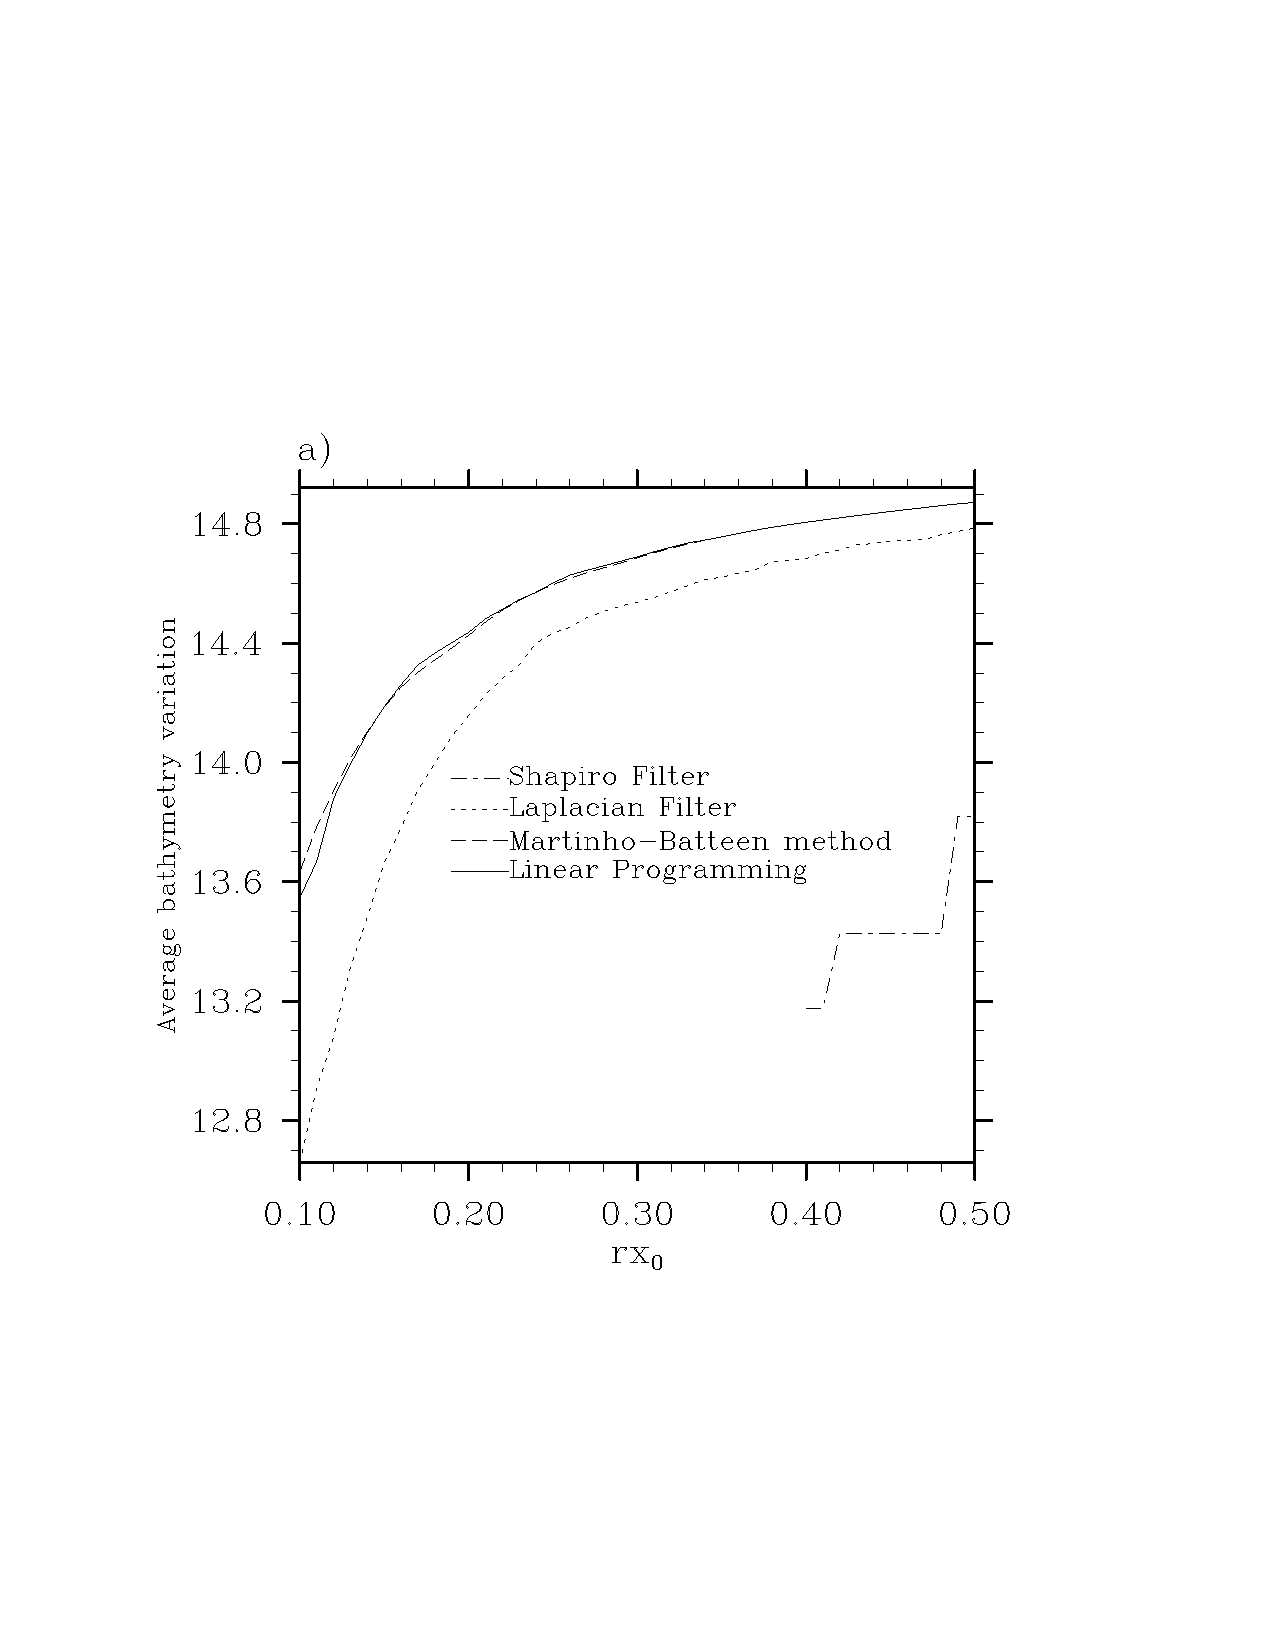
\epsfig{height=52mm, clip=, bb=74 182 484 566, file=OceanPic/ADRIA02_Gradient.pdf}\par
$60\times 160$
\end{minipage}
\begin{minipage}[b]{5.3cm}
\centering
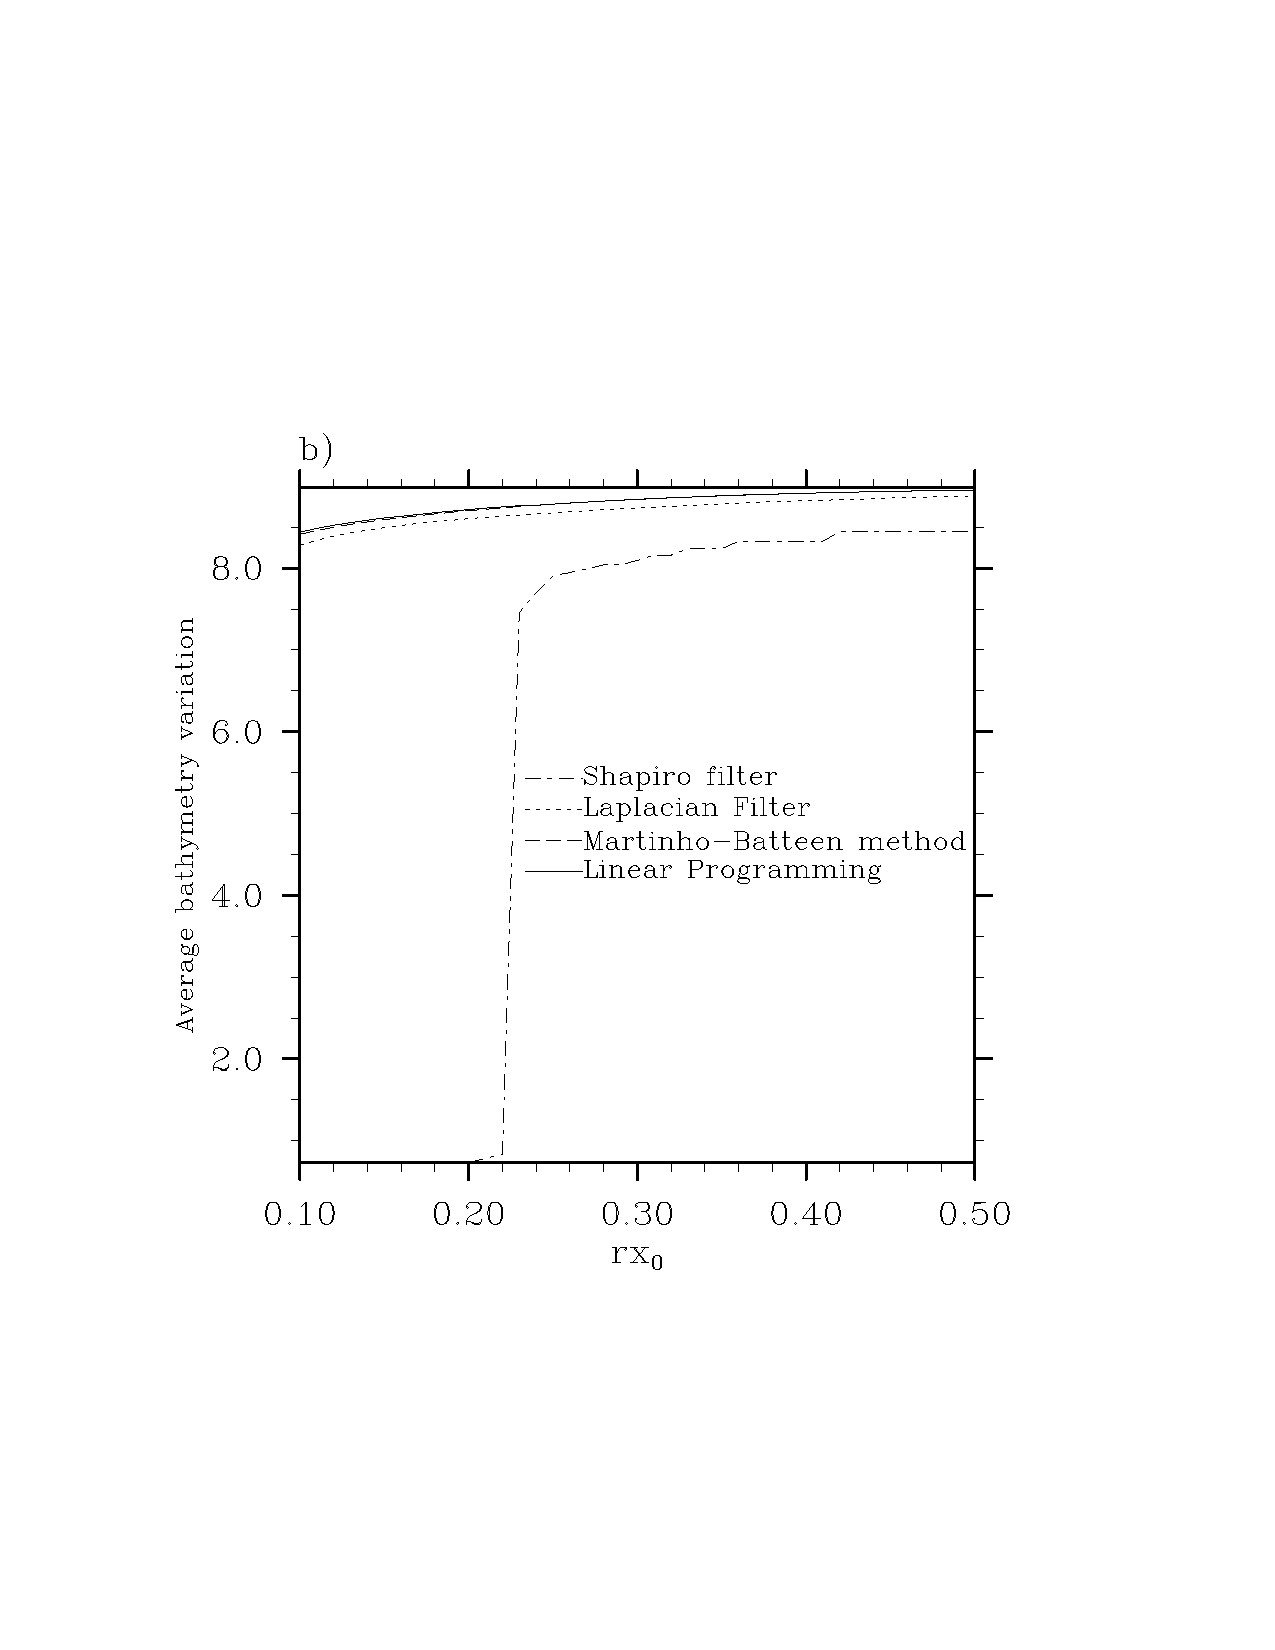
\epsfig{height=52mm, clip=, bb=101 182 484 566, file=OceanPic/VER10_NCOM2_Gradient.pdf}\par
$127\times 368$
\end{minipage}
\end{center}
The average variation of the bathymetry (m) from wet cell
to wet cell for bathymetry smoothing methods in terms of $rx_0(h)$
}



\frame{
  \frametitle{Average amplitude of bathymetry modification}

\begin{center}
\begin{minipage}[b]{5.3cm}
\centering
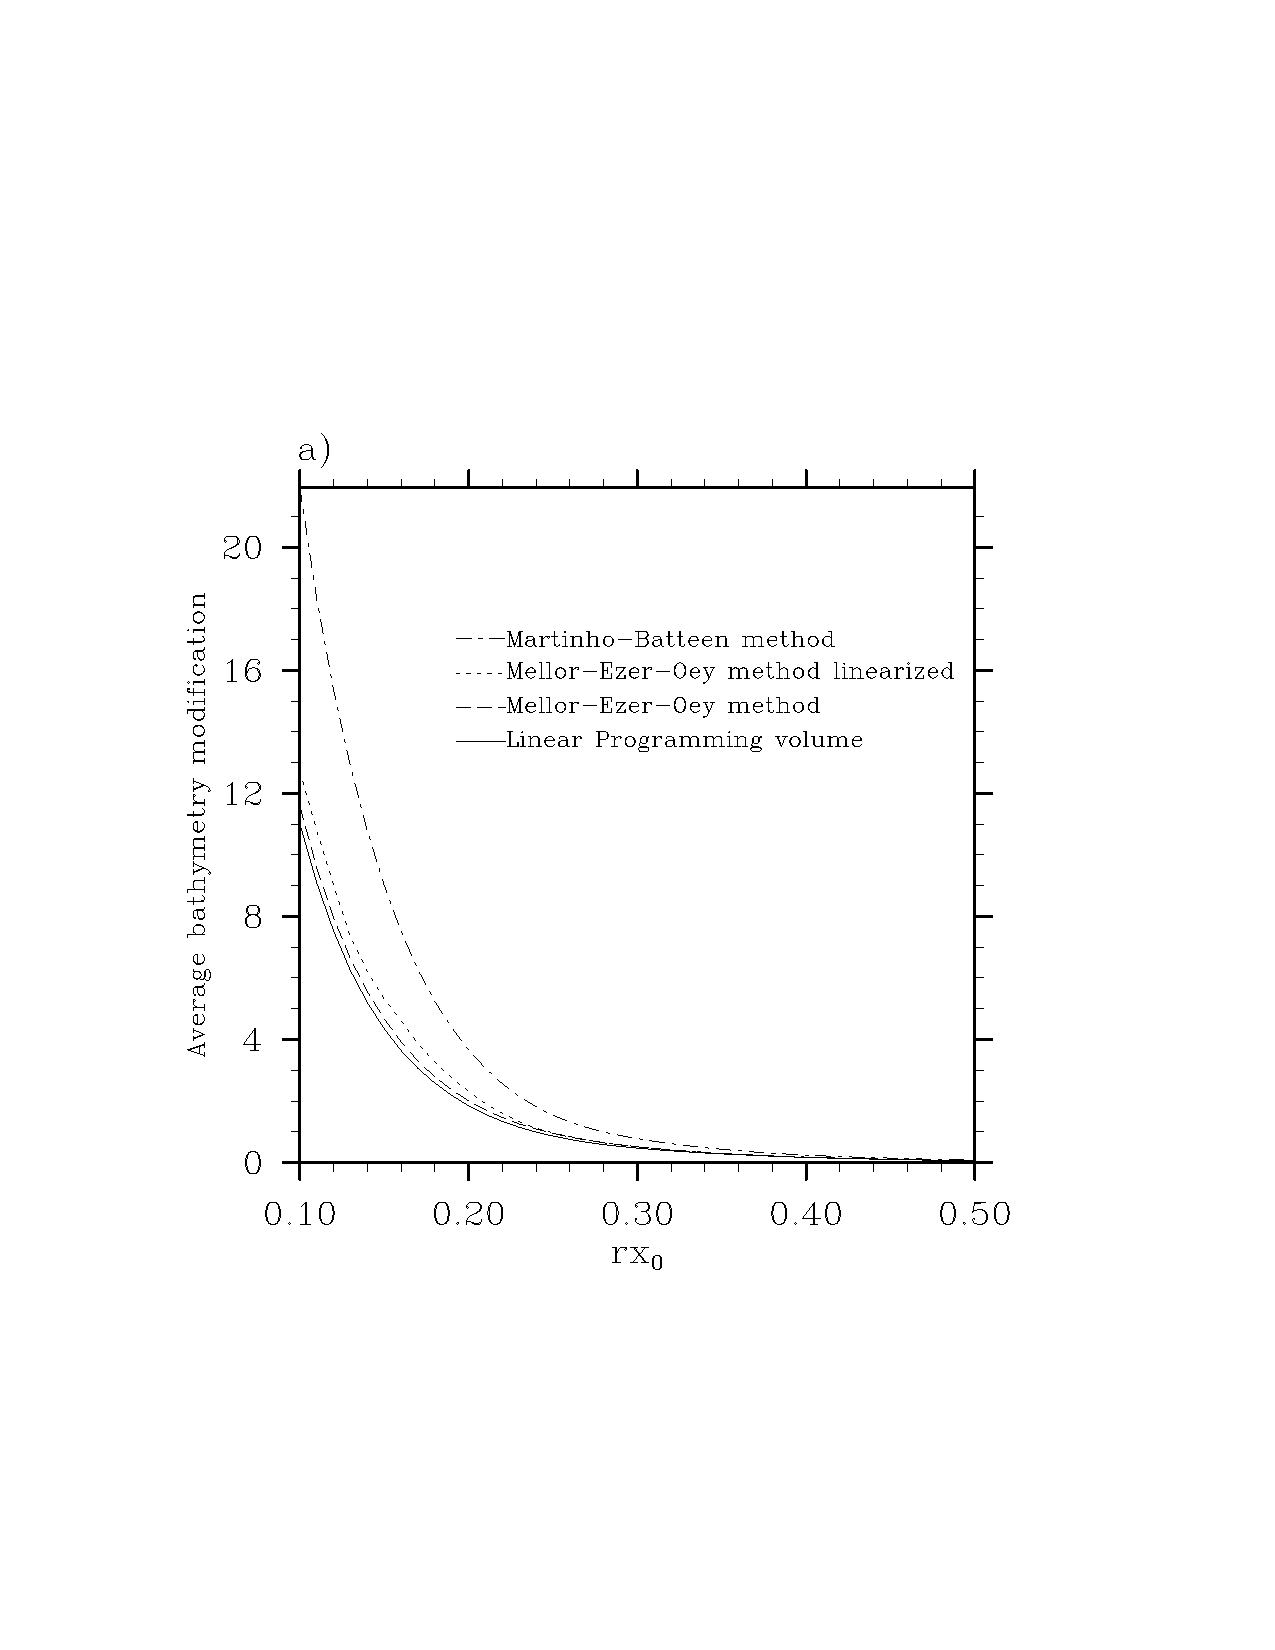
\epsfig{height=52mm, clip=, bb=90 182 476 569, file=OceanPic/ADRIA02_VolVarious.pdf}\par
$60\times 160$
\end{minipage}
\begin{minipage}[b]{5.3cm}
\centering
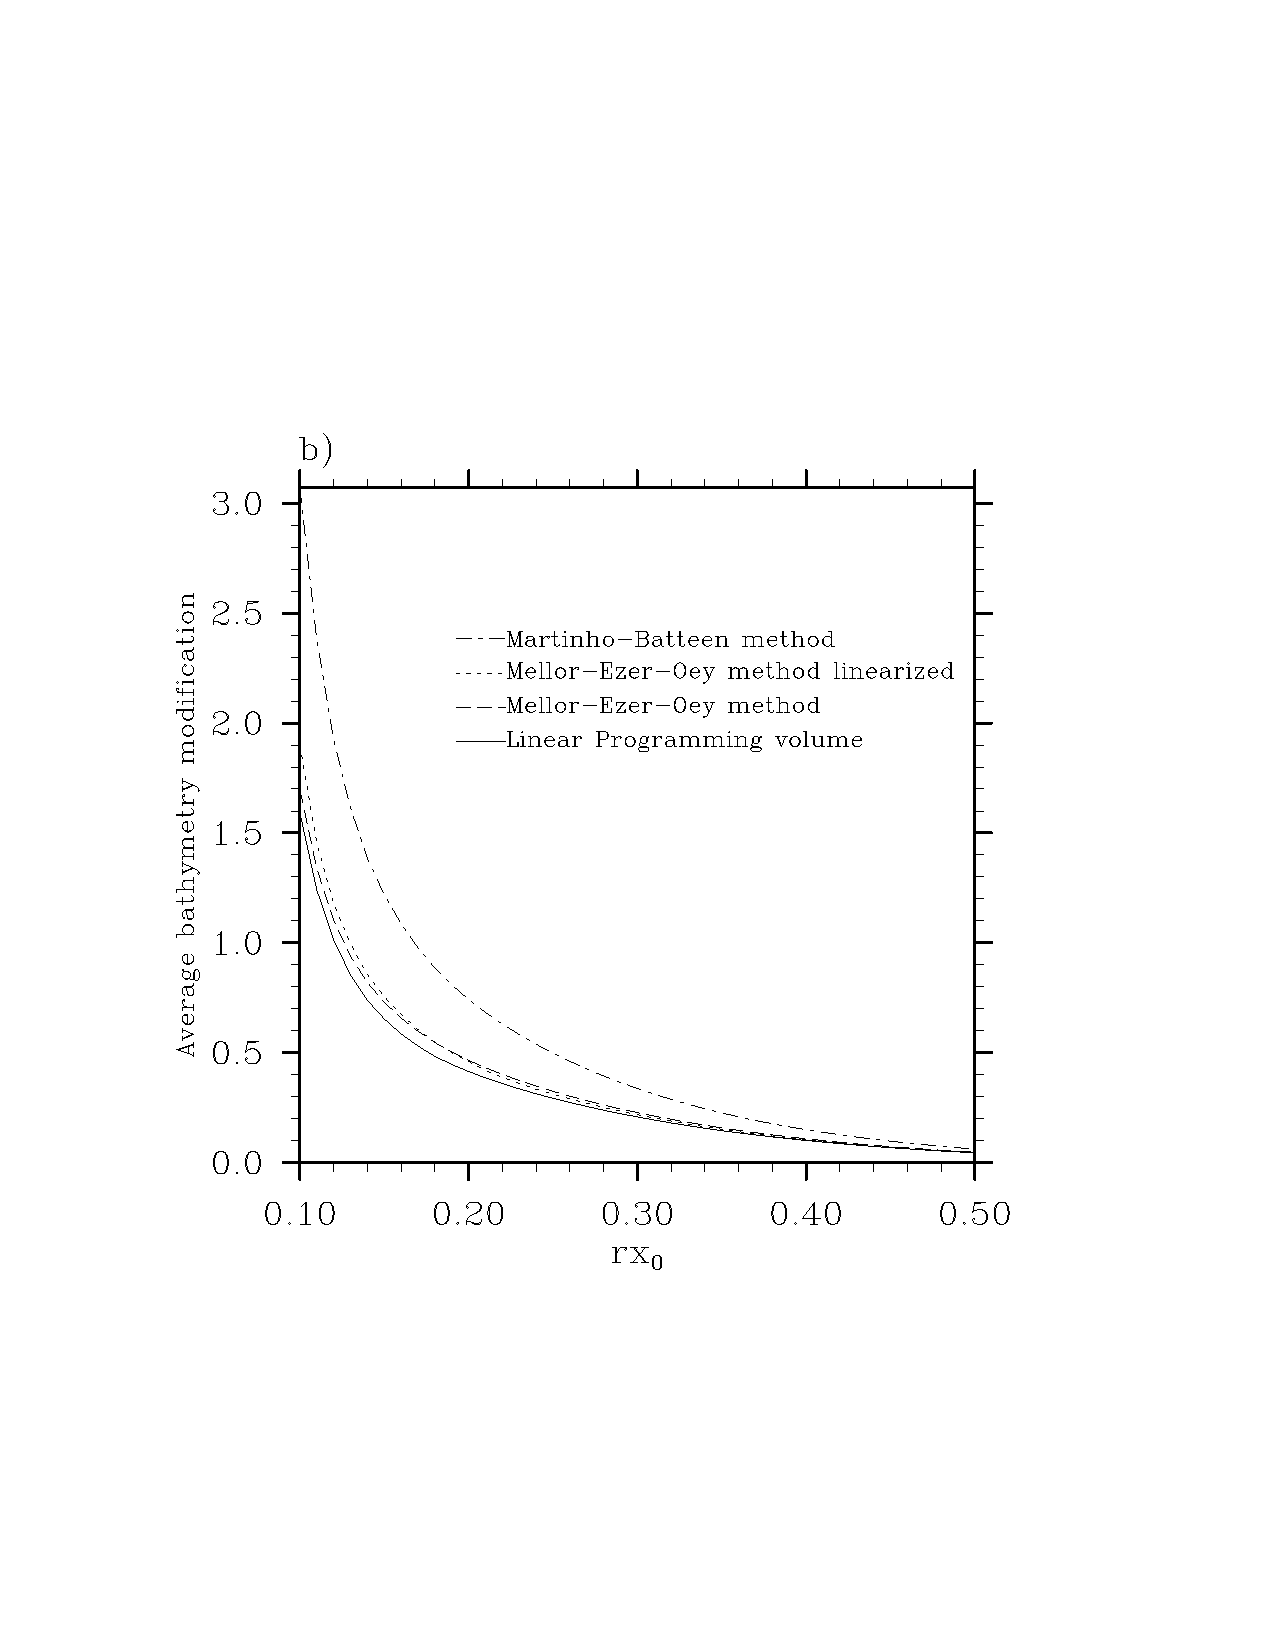
\epsfig{height=52mm, clip=, bb=101 182 485 569, file=OceanPic/VER10_NCOM2_VolVarious.pdf}\par
$127\times 368$
\end{minipage}
\end{center}
The average amplitude of bathymetry modification (m) in term of $rx_0$ for volume preserving smoothing methods
}

\frame{
  \frametitle{Average variation of the bathymetry}

\begin{center}
\begin{minipage}[b]{5.3cm}
\centering
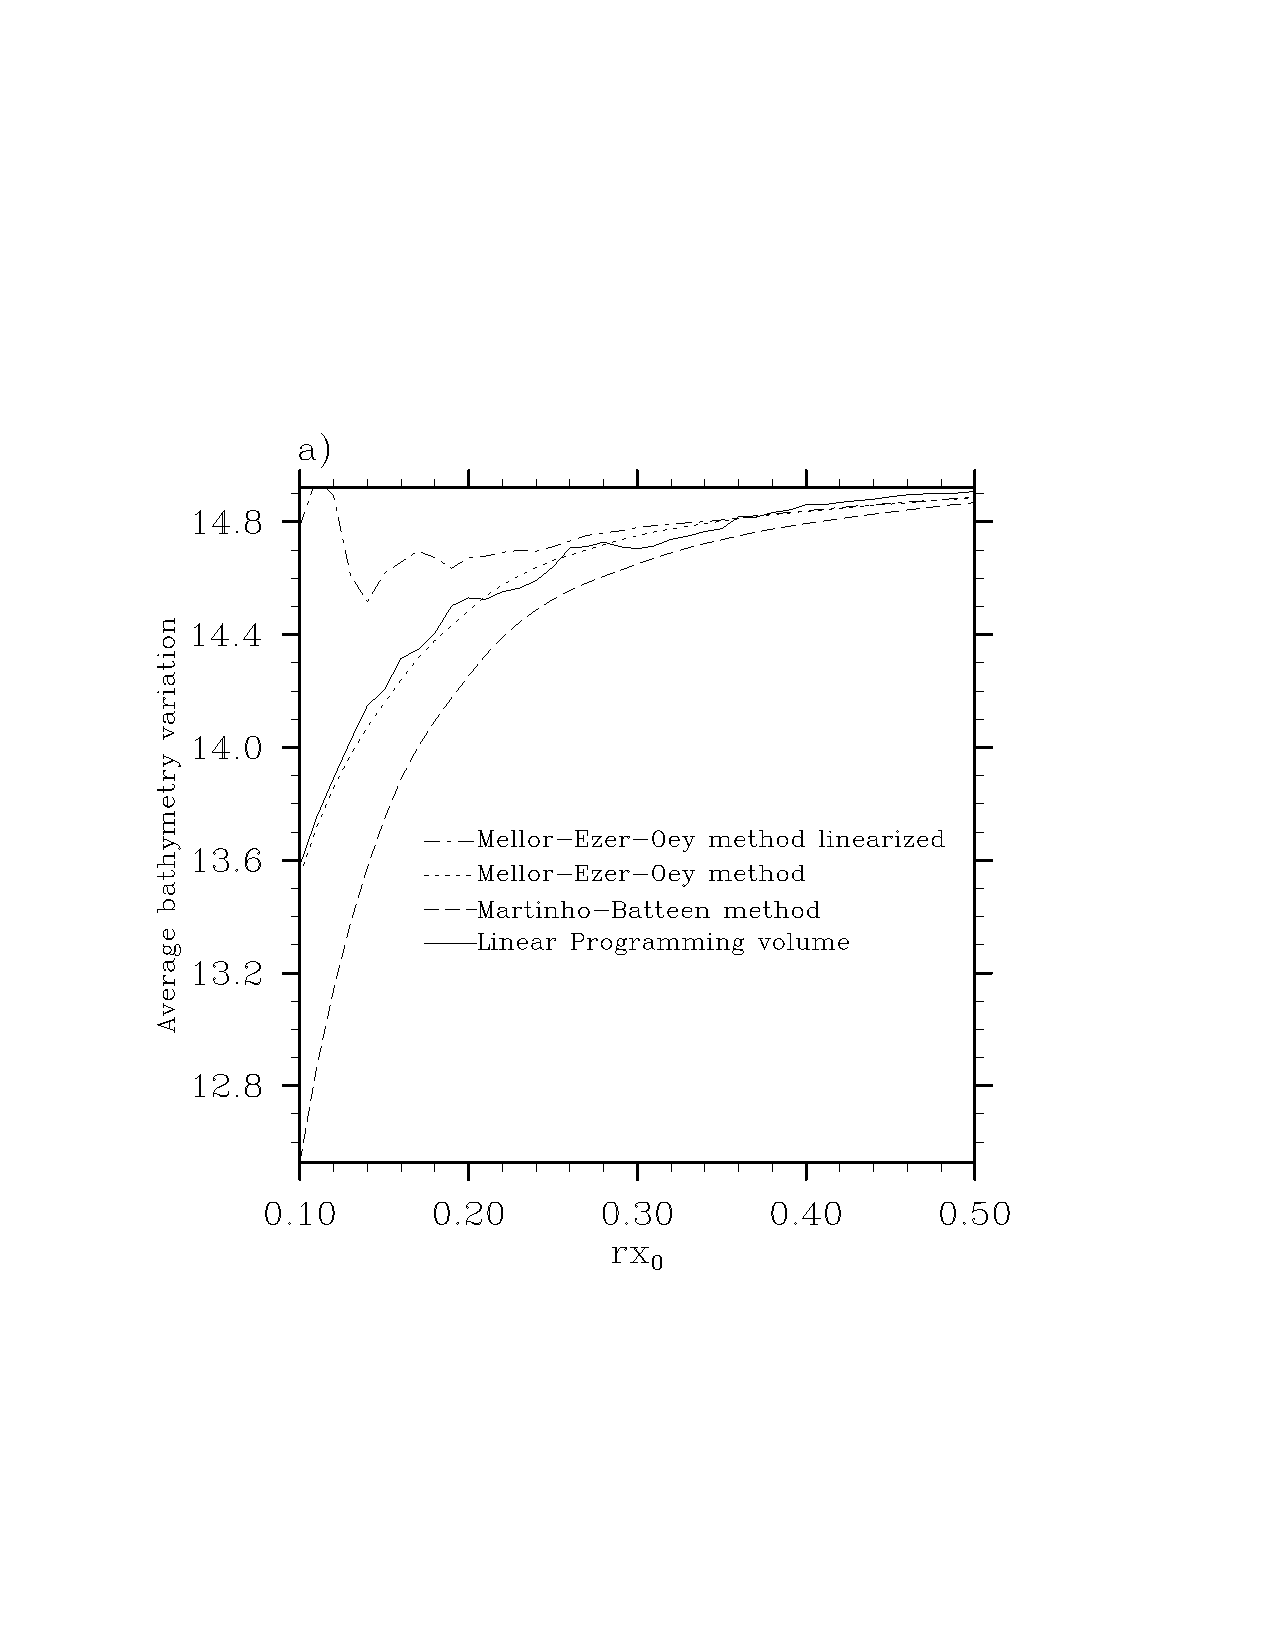
\epsfig{height=50mm, clip=, bb=75 182 484 566, file=OceanPic/ADRIA02_VolGradient.pdf}\par
$60\times 160$
\end{minipage}
\begin{minipage}[b]{5.3cm}
\centering
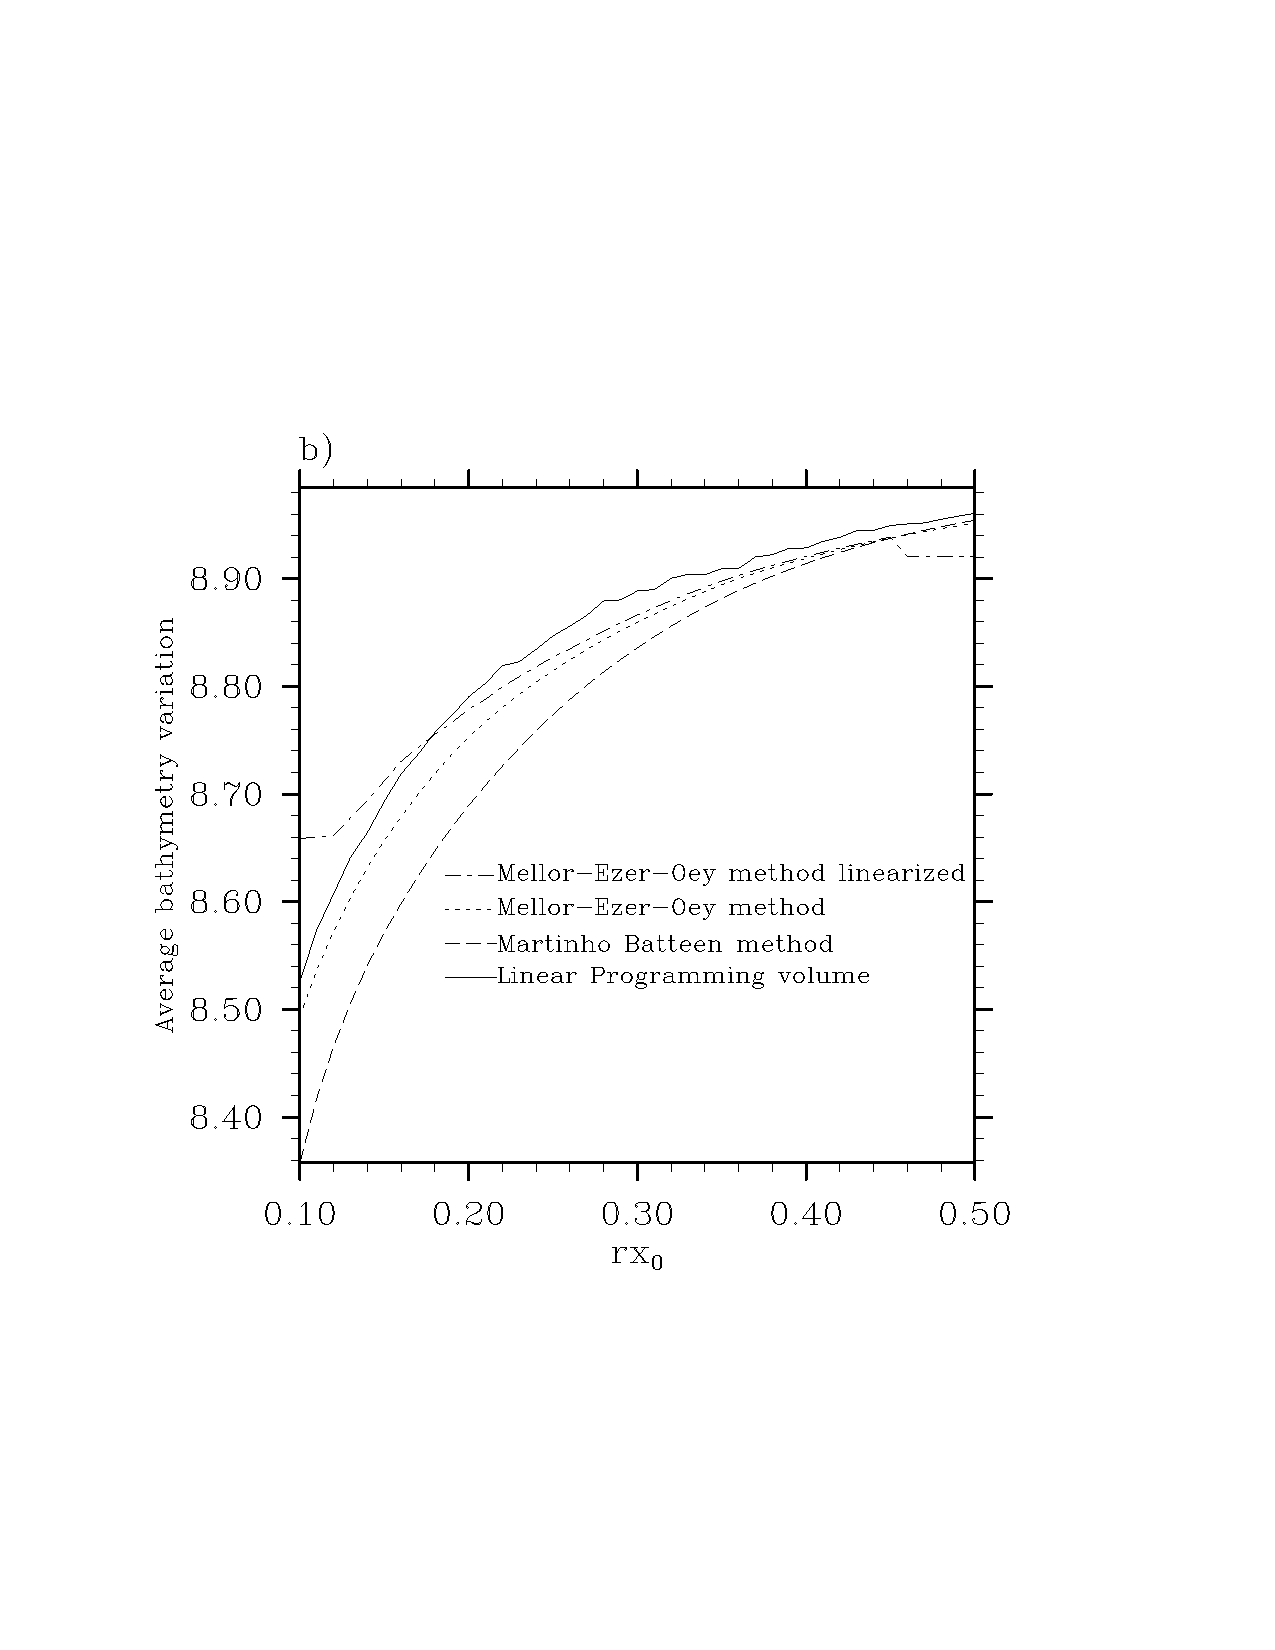
\epsfig{height=50mm, clip=, bb=91 182 484 566, file=OceanPic/VER10_NCOM2_VolGradient.pdf}\par
$127\times 368$
\end{minipage}
\end{center}
The average variation of the bathymetry (m) from wet cell
to wet cell for bathymetry smoothing methods preserving volume
in terms of $rx_0$
}


\frame{
  \frametitle{Stability of solutions}
What happens if one perturb by an infinitesimal quantity the observed bathymetry and/or the roughness factor?
\begin{itemize}
\item Heuristic methods are continuous.
\item Shapiro filter and Laplacian filter methods are not continuous.
\item Linear programming methods are not continuous since there are possible hoppings from one vertex to an adjacent one.
\end{itemize}
In practice during $0.01$ increments to $rx_0$,
\begin{itemize}
\item Shapiro/Laplacian filter are $10$ times more discontinuous than heuristic method.
\item polyhedral method are $2$ times more discontinuous.
\end{itemize}
}


\frame{
  \frametitle{Conclusions}

\begin{itemize}
\item Shapiro and Laplacian filter should be avoided since they create large perturbation of the bathymetry.
\item Heuristic methods like Martinho-Batteen, Mellor-Ezer-Oey work very well.
\item If $rx_0(h)\leq 0.2$ is needed, then linear programming might be what you need.
%\item There are many possible variants one can build on this to optimize the bathymetry.
\item All programs for optimizing over $rx_0$ or $rx_1$ are available from
\begin{center}
{\small \url{http://drobilica.irb.hr/~mathieu/Bathymetry/index.html}}
\end{center}

\end{itemize}
}





\frame{
\vspace{1.5cm}
\begin{center}
{\Huge \textcolor{red}{T}\textcolor{blue}{H}\textcolor{green}{A}\textcolor{blue}{N}\textcolor{red}{K}}\\[1cm]
{\Huge \textcolor{red}{Y}\textcolor{blue}{O}\textcolor{red}{U}}
%\epsfig{file=plit-gal10.eps, height=5.5cm}
\end{center}
}






\end{document}
